\scanpage{73}
% archive sheet number: 72

\[
\underline{G}(k')\handwritten{\longrightarrow}\underline{G}(k)\ .
\]
Ce dernier rend commutatif \inserted{(mod isomorphisme canonique)}\handwritten{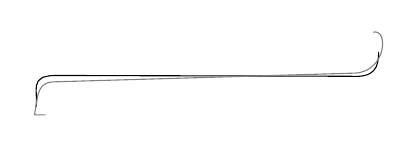
\begin{tikzpicture}[x=1cm,y=1cm,baseline=0cm]\draw[thin] (0,-.35)..controls (.03,-.15) and (-.1,.05)..(.25,.05)--(4,.04)..controls (4.3,.02) and (4.35,.15)..(4.35,.35);\draw[gray,thin] (.12,-.45)--(-.02,-.45)..controls (.03,-.15) and (.02,-.03)..(.26,-.03)--(4.05,.08)..controls (4.45,.1) and (4.48,.65)..(4.28,.6);\end{tikzpicture}} le diagramme
\diagram{\begin{tikzcd}[ampersand replacement=\&,column sep=large,row sep=large]
\underline{G}(k\handwritten{'}) \handwritten{\arrow[r]} \handwritten{\arrow[d,draw=none,"{
\begin{tikzpicture}[x=1cm,y=1cm,baseline=0cm]\draw[thick] (0,.7)--(.025,-.5)..controls (.02,-.62) and (-.1,-.63)..(-.08,-.53);\fill (-.035,-.56) circle (.035);\end{tikzpicture}}" description]} \& \underline{G}(k^{\deleted{\unsure{'}}}) \handwritten{\arrow[d,draw=none,"{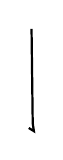
\begin{tikzpicture}[x=1cm,y=1cm,baseline=0cm]\draw[thick] (0,.7)--(.015,-.5)--(.03,-.6)--(-.035,-.56);\end{tikzpicture}}" description]} \\
\handwritten{\underline{\pi}_{p}}(k')\mathrm{x}\handwritten{[}G_m\handwritten{]}_{\underline{\unsure{\mathbb{Q}|Q}}_p} \handwritten{\arrow[r]} \& \handwritten{\underline{\unsure{\pi|\Pi}}}_p(k)\mathrm{x}\handwritten{[}\underline{G}_m\handwritten{]}_{\underline{Q}_p}
\end{tikzcd}}
(i.e. on a, sur les catégories tannakiennes\deleted{, un} correspondantes, un diag\unsure{\deleted{r}g|\deleted{g}r}amme comm\unsure{\deleted{u}y|\deleted{y}u}tatif à isomorphisme \inserted{can.}\handwritten{\begin{tikzpicture}[x=1cm,y=1cm,baseline=0cm]\draw[thin] (0,-.25)..controls (.12,.12) and (.3,.2)..(.6,.28)..controls (.9,.35) and (1.1,.4)..(1.18,.62);\end{tikzpicture}} près).

Oubliant dans ce dernier les facteurs 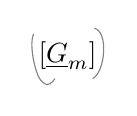
\begin{tikzpicture}[baseline=(f.base),x=1cm,y=1cm]\node[inner sep=0pt] (f) {$\handwritten{[}\underline{G}_m\handwritten{]}$};\draw[gray,thin] (-.43,.28)..controls (-.5,.14) and (-.4,-.3)..(-.31,-.34)..controls (-.24,-.4) and (-.2,-.34)..(-.16,-.29);\draw[gray,thin] (.34,.35)..controls (.52,.31) and (.48,-.2)..(.32,-.29);\end{tikzpicture}, on voit donc que $\underline{G}(k')\handwritten{\longrightarrow}\underline{G}(k)$ se factorise par la sous-\deleted{catégorie} gerbe de $\underline{G}(k)$ correspondant au sous-groupe fermé de $\handwritten{\pi}_1(k)$ image de $\handwritten{\pi}_1(k')$ ... A prouver:

\uline{Proposition} \handwritten{6.1.} Si $k'$ est une extension \deleted{finie} étale de $k$, alors l'homomorphisme de gerbes $\underline{G}(k')\handwritten{\longrightarrow}\underline{G}(k)$ est un \uline{monomorphisme} dont l'image est exactement la sous-gerbe ``ouverte'' définie ci-dessus. En particulie\unsure{\deleted{r}t|\deleted{t}r}, si $k'$ est une extension finie galoisienne de $k$, \deleted{on a une} de groupe de \raisebox{.4ex}{G}alois $g$, et on une suite exacte canonique de gerbes
\[
0\handwritten{\longrightarrow}\underset{\handwritten{\unsure{\mu|\deleted{\mu}|\pi|\deleted{\pi}}}}{\underline{G}^{\deleted{\unsure{'}}}}(k\handwritten{'})\handwritten{\longrightarrow}\underline{G}(k)\handwritten{\mathrel{\begin{tikzpicture}[baseline=0cm,x=1cm,y=1cm]\draw[thick] (0,0)--(.6,0);\draw[thick] (.55,0)--(.55,-.04);\end{tikzpicture}}}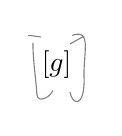
\begin{tikzpicture}[baseline=(f.base),x=1cm,y=1cm]\node[inner sep=0pt] (f) {$\handwritten{[}g\handwritten{]}$};\draw[gray,thin] (-.2,.35)--(-.36,.37);\draw[gray,thin] (-.3,.27)..controls (-.3,.04) and (-.26,-.2)..(-.25,-.38)..controls (-.24,-.51) and (-.06,-.4)..(-.05,-.33);\draw[gray,thin] (.2,.37)..controls (.46,.46) and (.33,.12)..(.35,-.2)..controls (.35,-.55) and (.2,-.52)..(.17,-.35);\draw[gray,thin] (.17,.26)--(.35,.36);\end{tikzpicture}_{\underline{Q}_p}\handwritten{\longrightarrow}0\ .
\]
Cet énoncé devrait être formellement équivalent au suivant: $\operatorname{Spec}(k')\handwritten{\longrightarrow}\operatorname{Spec}(k)$ est un morphisme de descente effective pour la catégorie fibrée des $\mathrm{Fcriso}(L)$ sur des composés finis\inserted{$L$}\handwritten{\begin{tikzpicture}[x=1cm,y=1cm,baseline=0cm]\draw[thin] (0,-.3)..controls (.01,.02) and (.33,.3)..(.5,.48)..controls (.68,.65) and (.8,.74)..(.74,.88);\end{tikzpicture}} de corps de car. $p$. La démonstration de ce dernier fait est $\handwritten{\pm}$ triviale.

\uline{Question} \handwritten{6.2.} A-t-on encore un énoncé analogue lorsqu'on suppose que $k'$ est une extension galoisienne de $k$ qui peut-être infinie ? Le cas le plus intéressant serait celui où $k'$est la clôture séparable de $k$, de sorte qu'on aurait un dévissage de $\underline{G}(k)$ en
\[
0\handwritten{\longrightarrow}\underline{G}(\handwritten{\bar{k}}^{\deleted{\unsure{'}}})\handwritten{\longrightarrow}\underline{G}(k)\handwritten{\longrightarrow\underline{\unsure{\pi|\Pi}}}_p(k)\handwritten{\longrightarrow}0\quad\deleted{\unsure{?}}\ ;
\tag*{\handwritten{(\unsure{6}.2.1)}}
\]
lorsque $k$ est parfait i.e. $\handwritten{\bar{k}}$ alg. clos, nous verrons que $\underline{G}(\handwritten{\bar{k}})$ ne dépend pas essentiellement de \handwritten{$k$. À}

\mspage{72}
